%%%%%%%%%%%%%%%%%%%%%%%%%%%%%%%%%%%%%%%%%
% Journal Article
% LaTeX Template
% Version 1.4 (15/5/16)
%
% This template has been downloaded from:
% http://www.LaTeXTemplates.com
%
% Original author:
% Frits Wenneker (http://www.howtotex.com) with extensive modifications by
% Vel (vel@LaTeXTemplates.com)
%
% License:
% CC BY-NC-SA 3.0 (http://creativecommons.org/licenses/by-nc-sa/3.0/)
%
%%%%%%%%%%%%%%%%%%%%%%%%%%%%%%%%%%%%%%%%%

%----------------------------------------------------------------------------------------
%	PACKAGES AND OTHER DOCUMENT CONFIGURATIONS
%----------------------------------------------------------------------------------------

\documentclass[10pt]{article} % Single column

%\documentclass[twoside,twocolumn]{article} % Two column

\usepackage{blindtext} % Package to generate dummy text throughout this template 

\usepackage[sc]{mathpazo} % Use the Palatino font
\usepackage[T1]{fontenc} % Use 8-bit encoding that has 256 glyphs
\linespread{1.05} % Line spacing - Palatino needs more space between lines
\usepackage{microtype} % Slightly tweak font spacing for aesthetics

\usepackage[spanish]{babel} % Language hyphenation and typographical rules

\usepackage[hmarginratio=1:1,top=32mm,columnsep=20pt]{geometry} % Document margins
\usepackage[hang, small,labelfont=bf,up,textfont=it,up]{caption} % Custom captions under/above floats in tables or figures
\usepackage{booktabs} % Horizontal rules in tables

\usepackage{lettrine} % The lettrine is the first enlarged letter at the beginning of the text

\usepackage{enumitem} % Customized lists
\setlist[itemize]{noitemsep} % Make itemize lists more compact

\usepackage{abstract} % Allows abstract customization
\renewcommand{\abstractnamefont}{\normalfont\bfseries} % Set the "Abstract" text to bold
\renewcommand{\abstracttextfont}{\normalfont\small\itshape} % Set the abstract itself to small italic text

\usepackage{titlesec} % Allows customization of titles
\renewcommand\thesection{\Roman{section}} % Roman numerals for the sections
\renewcommand\thesubsection{\roman{subsection}} % roman numerals for subsections
\titleformat{\section}[block]{\large\scshape\centering}{\thesection.}{1em}{} % Change the look of the section titles
\titleformat{\subsection}[block]{\large}{\thesubsection.}{1em}{} % Change the look of the section titles

\usepackage{fancyhdr} % Headers and footers
\pagestyle{fancy} % All pages have headers and footers
\fancyhead{} % Blank out the default header
\fancyfoot{} % Blank out the default footer
\fancyhead[C]{Lenguajes de Programaci\'on: \textbf{Concurrencia}} % Custom header text
\fancyfoot[RO,LE]{\thepage} % Custom footer text

\usepackage{titling} % Customizing the title section

\usepackage{hyperref} % For hyperlinks in the PDF

\usepackage{graphicx} % For images

\usepackage{pifont} % bullets

% Keywords command
\providecommand{\keywords}[1]
{
	\small	
	\vspace{0.5em}
	\noindent \textbf{\textit{Palabras clave --- }} #1
}


%----------------------------------------------------------------------------------------
%	TITLE SECTION
%----------------------------------------------------------------------------------------

\setlength{\droptitle}{-4\baselineskip} % Move the title up

\pretitle{\begin{center}\Huge\bfseries} % Article title formatting
\posttitle{\end{center}} % Article title closing formatting
\title{\normalsize{Lenguajes de Programaci\'on}\\
\Huge\bfseries Concurrencia\\

\includegraphics[height=5em]{go_cs_logo.png}} % Article title
\author{% 
\normalsize\textsc{Leandro Rodr\'iquez Llosa}\\
\normalsize\textsc{Laura V. Riera P\'erez}\\ 
\normalsize\textsc{Marcos M. Tirador del Riego} \\[2ex]
\small Tercer a\~no. Ciencias de la Computaci\'on. \\ % institution
\small Facultad de Matem\'atica y Computaci\'on, Universidad de La Habana, Cuba \\ % institution
}
\date{\footnotesize Noviembre 2022 } % Leave empty to omit a date


% Abstract configurations
\renewenvironment{abstract}
{\small
	\begin{center}
		\bfseries \abstractname\vspace{-.5em}\vspace{0pt}
	\end{center}
	\list{}{
		\setlength{\leftmargin}{1.5cm}%
		\setlength{\rightmargin}{\leftmargin}%
	}%
	\item\relax}
{\endlist}


\usepackage{todonotes} % \TODO
\usepackage{listings} % Code listings
\usepackage{xcolor}
\definecolor{backcolour}{rgb}{0.95,0.95,0.92}

\newcommand{\csl}[1]{\colorbox{backcolour}{\texttt{#1}}}

\newcommand{\imgcaption}[2]{\tiny \textbf{Figura #1.} #2.}

\newcommand{\mgc}[2][]{\colorbox{backcolour}{\texttt{\_\_#2\_\_#1}}}

\newcommand{\mgccapt}[1]{\texttt{\_\_#1\_\_}}

% Hyperlinks configurations
\hypersetup{
	colorlinks=true,
	linkcolor=black,
	filecolor=magenta,      
	urlcolor=cyan,
	pdftitle={Overleaf Example},
	pdfpagemode=FullScreen,
}

%----------------------------------------------------------------------------------------

\begin{document}
% Print the title
\maketitle

%----------------------------------------------------------------------------------------
%	ARTICLE CONTENTS
%----------------------------------------------------------------------------------------

\section{Concurrencia y paralelismo}

La \textit{concurrencia} es la ejecuci\'on simult\'anea de varias hebras\footnote{Una hebra es una ejecuci\'on secuencial de instrucciones.}, pero esta simultaneidad puede ser solo en apariencia. Los procesos tienen lugar en el mismo tiempo, pero la ejecución de todos ellos no ocurre en el mismo instante. En un momento dado solo se ejecuta un programa, y este lo hace de forma secuencial en un tiempo limitado establecido para realizar sus operaciones. Si este no termina su ejecuci\'on dentro de su tiempo, es puesto en espera, d\'andole paso al p\'oximo, y es resumido una vez vuelva a tocar su tiempo. Sea T el tiempo total de ejecuci\'on de dos programas concurrentes $ P_{1} $ y $ P_{2} $: 

\begin{center}
	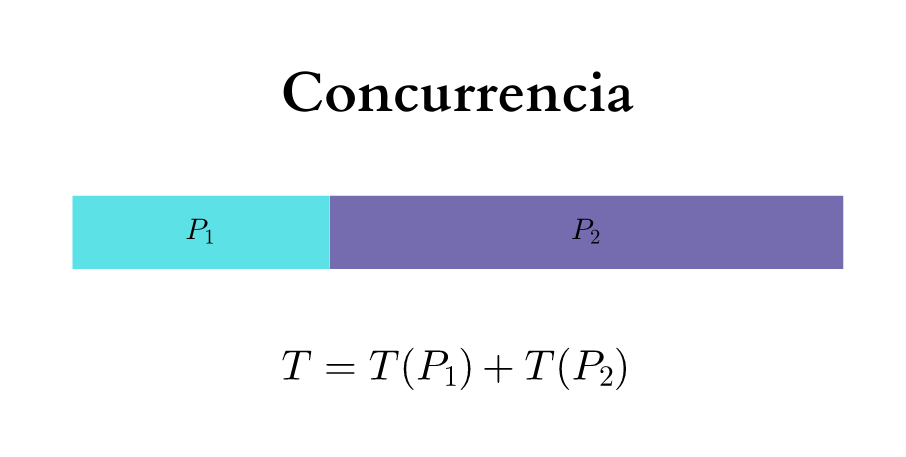
\includegraphics[width=5cm]{concurrencia.png}
\end{center}

En el \textit{paralelismo} la ejecución ocurre en el mismo instante físico, los c\'alculos se realizan de forma verdaderamente simul\'anea. Para maximizar el uso de múltiples procesadores o n\'ucleos, presentes en las CPU modernas, el procesamiento en paralelo dividirá el trabajo entre varios subprocesos, cada uno de los cuales puede ejecutarse de forma independiente en un núcleo diferente. Paralelismo implica concurrencia, pero no se cumple el rec\'iproco. Sea ahora T el tiempo total de ejecuci\'on de dos programas paralelos $ P_{1} $ y $ P_{2} $:

\begin{center}
	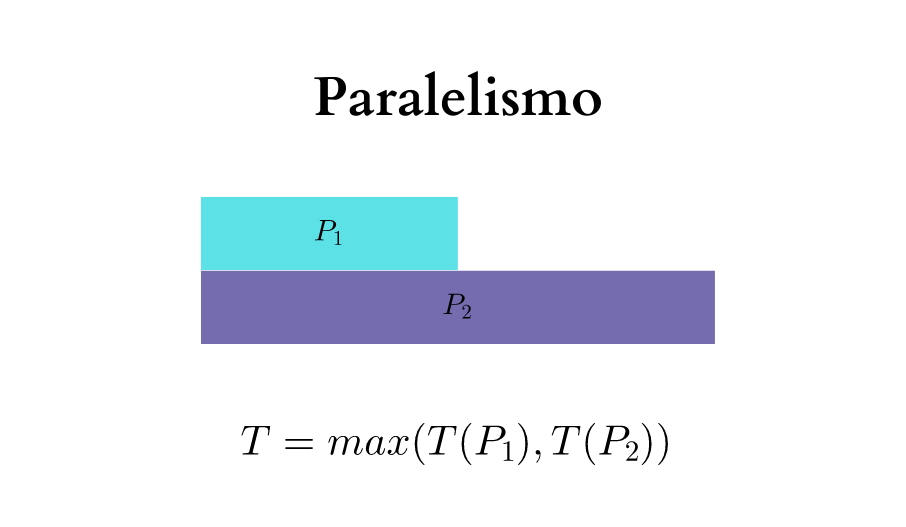
\includegraphics[width=5cm]{paralelismo.png}
\end{center}

En la programaci\'on concurrente ocurre con frecuencia que las hebras que se ejecuten necesiten sincronizar e intercambiar informaci\'on enn alg\'un momento, lo cual se hace usualmente a trav\'es de memoria compartida. Esto puede causar problemas dado que varios procesos estar\'an realizando modificaciones concurrentemente sobre la misma memoria. M\'ultiples hebras se encuentran en una \textit{condici\'on de carrera} si el resultado de su ejecuci\'on depende del orden en que se ejecutan las instrucciones que componen cada hebra. 

Se denomina \textit{sección crítica} a la porción de código de una hebra en la que se accede a un recurso compartido y que puede entrar en una condici\'on de carrera, por lo que no debe ser accedido por más de un proceso o hilo en ejecución a la vez. Se necesita un mecanismo de sincronización en la entrada y salida de la sección crítica para asegurar la utilización exclusiva del recurso. Los recursos destinados a lograr este comportamiento se denominan de exclusi\'on mutua o \textit{mutex}. Los m\'as comunes son los candados, monitores y semáforos.

\subsection{Locks en C\#}

Los candados garantizan acceso exclusivo a un recurso compartido. La sincronizaci\'on se logra poni\'endole el candado a una variable. En C\# esto se logra mediante la palabra reservada \csl{lock}. 

El candado de exclusi\'on mutua es adquirido para un objeto dado por \csl{lock}, se ejecuta el bloque de c\'odigo dentro de su cuerpo y luego se libera el candado. Mientras un hilo mantenga un candado, este puede volver a adquirirlo y liberarlo. Cualquier otro subproceso no puede adquirir el candado y debe esperar hasta que este sea liberado. A continuaci\'on se muestra la forma de declarar un candado:

\begin{center}
	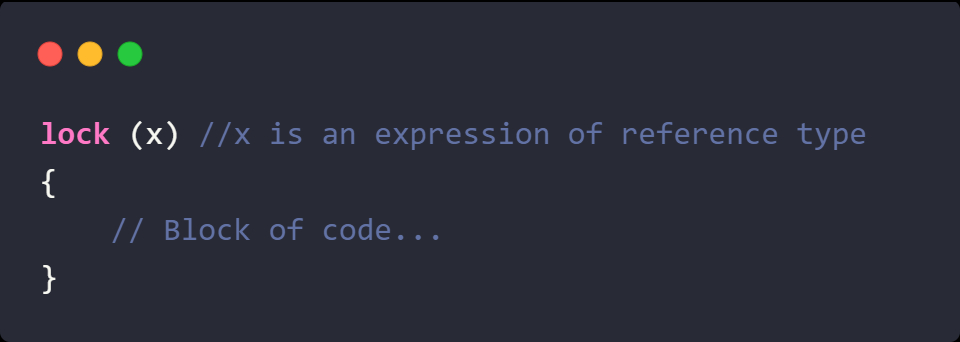
\includegraphics[width=8cm]{lock.jpg}
\end{center}

\csl{lock} controla toda una secci\'on sin dejar libertad para adquirir o liberar un recurso basado en una l\'ogica m\'as propia del problema a solucionar. 

\subsection{Monitors en C\#}

La clase Monitor permite sincronizar el acceso a una región de código tomando y liberando un bloqueo en un objeto determinado llamando a los métodos Monitor.Enter, Monitor.TryEnter y Monitor.Exit . Los bloqueos de objeto proporcionan la capacidad de restringir el acceso a un bloque de código, normalmente denominado sección crítica. Aunque un subproceso posee el bloqueo de un objeto, ningún otro subproceso puede adquirir ese bloqueo. También puede usar la Monitor clase para asegurarse de que ningún otro subproceso pueda acceder a una sección del código de aplicación que ejecuta el propietario del bloqueo, a menos que el otro subproceso ejecute el código mediante un objeto bloqueado diferente.

\subsection{Semaphores en C\#}

Un sem\'aforo limita la cantidad de subprocesos que pueden acceder a un recurso o conjunto de recursos al mismo tiempo. En C\# puede ser encontrado en la clase \csl{System.Threading.Semaphore}.

Cuenta con dos propiedades fundamentales: \csl{Count}, que indica el n\'umero de hilos que pueden ingresar al sem\'aforo en este momento; y \csl{InitialCount}, que indica la cantidad m\'axima de hilos que pueden ingresar al sem\'aforo. Los subprocesos ingresan al semáforo llamando al método \csl{WaitOne()}, y liberan el semáforo llamando al método \csl{Release()}.

El \csl{Count} en un semáforo se reduce cada vez que un subproceso ingresa al semáforo y se incrementa cuando un subproceso libera el semáforo. Cuando el \csl{Count} es cero, las solicitudes posteriores se bloquean hasta que otros subprocesos liberan el semáforo; no hay un orden predeterminado en el que los subprocesos bloqueados entren en el semáforo. Cuando todos los subprocesos han liberado el semáforo, el \csl{Count} estar\'a en el valor máximo especificado cuando se creó el semáforo (\csl{InitialCount}).

Un subproceso puede ingresar el semáforo varias veces llamando al método \csl{WaitOne()}; repetidamente. Para liberar algunas o todas estas entradas, el subproceso puede llamar a la sobrecarga del método \csl{Release()} sin parámetros varias veces, o puede llamar a la sobrecarga del método \csl{Release(int)} que especifica la cantidad de entradas que se liberarán.

No se aplica la identidad del subproceso en las llamadas a \csl{WaitOne()} o \csl{Release()}, por lo que es responsabilidad del programador asegurarse de que los subprocesos no liberen el semáforo m\'as veces de las requeridas. Por ejemplo, si un semáforo tiene un recuento máximo de dos y que tanto el hilo A como el hilo B entran en el semáforo. Si un error de programación en el subproceso B hace que llame a Release dos veces, ambas llamadas se realizan correctamente. El conteo en el semáforo estar\'a lleno, y cuando el subproceso A eventualmente llame a Release, se lanzar\'a una excepci\'on SemaphoreFullException.

Un sem\'aforo puede ser de dos tipos: local o nombrado del sistema. Un semáforo local existe solo dentro de su proceso, pudiendo ser utilizado por cualquier subproceso en este que tenga una referencia al mismo. Cada objeto Semaphore es un semáforo local independiente. Por otro lado, si se crea un objeto Semaphore utilizando un constructor que acepta un nombre, se asocia con un semáforo del sistema operativo de ese nombre, siendo visible en todo el sistema operativo y puediendo utilizarse para sincronizar las actividades de los procesos. Se puede usar el método OpenExisting para abrir un semáforo nombrado del sistema existente.

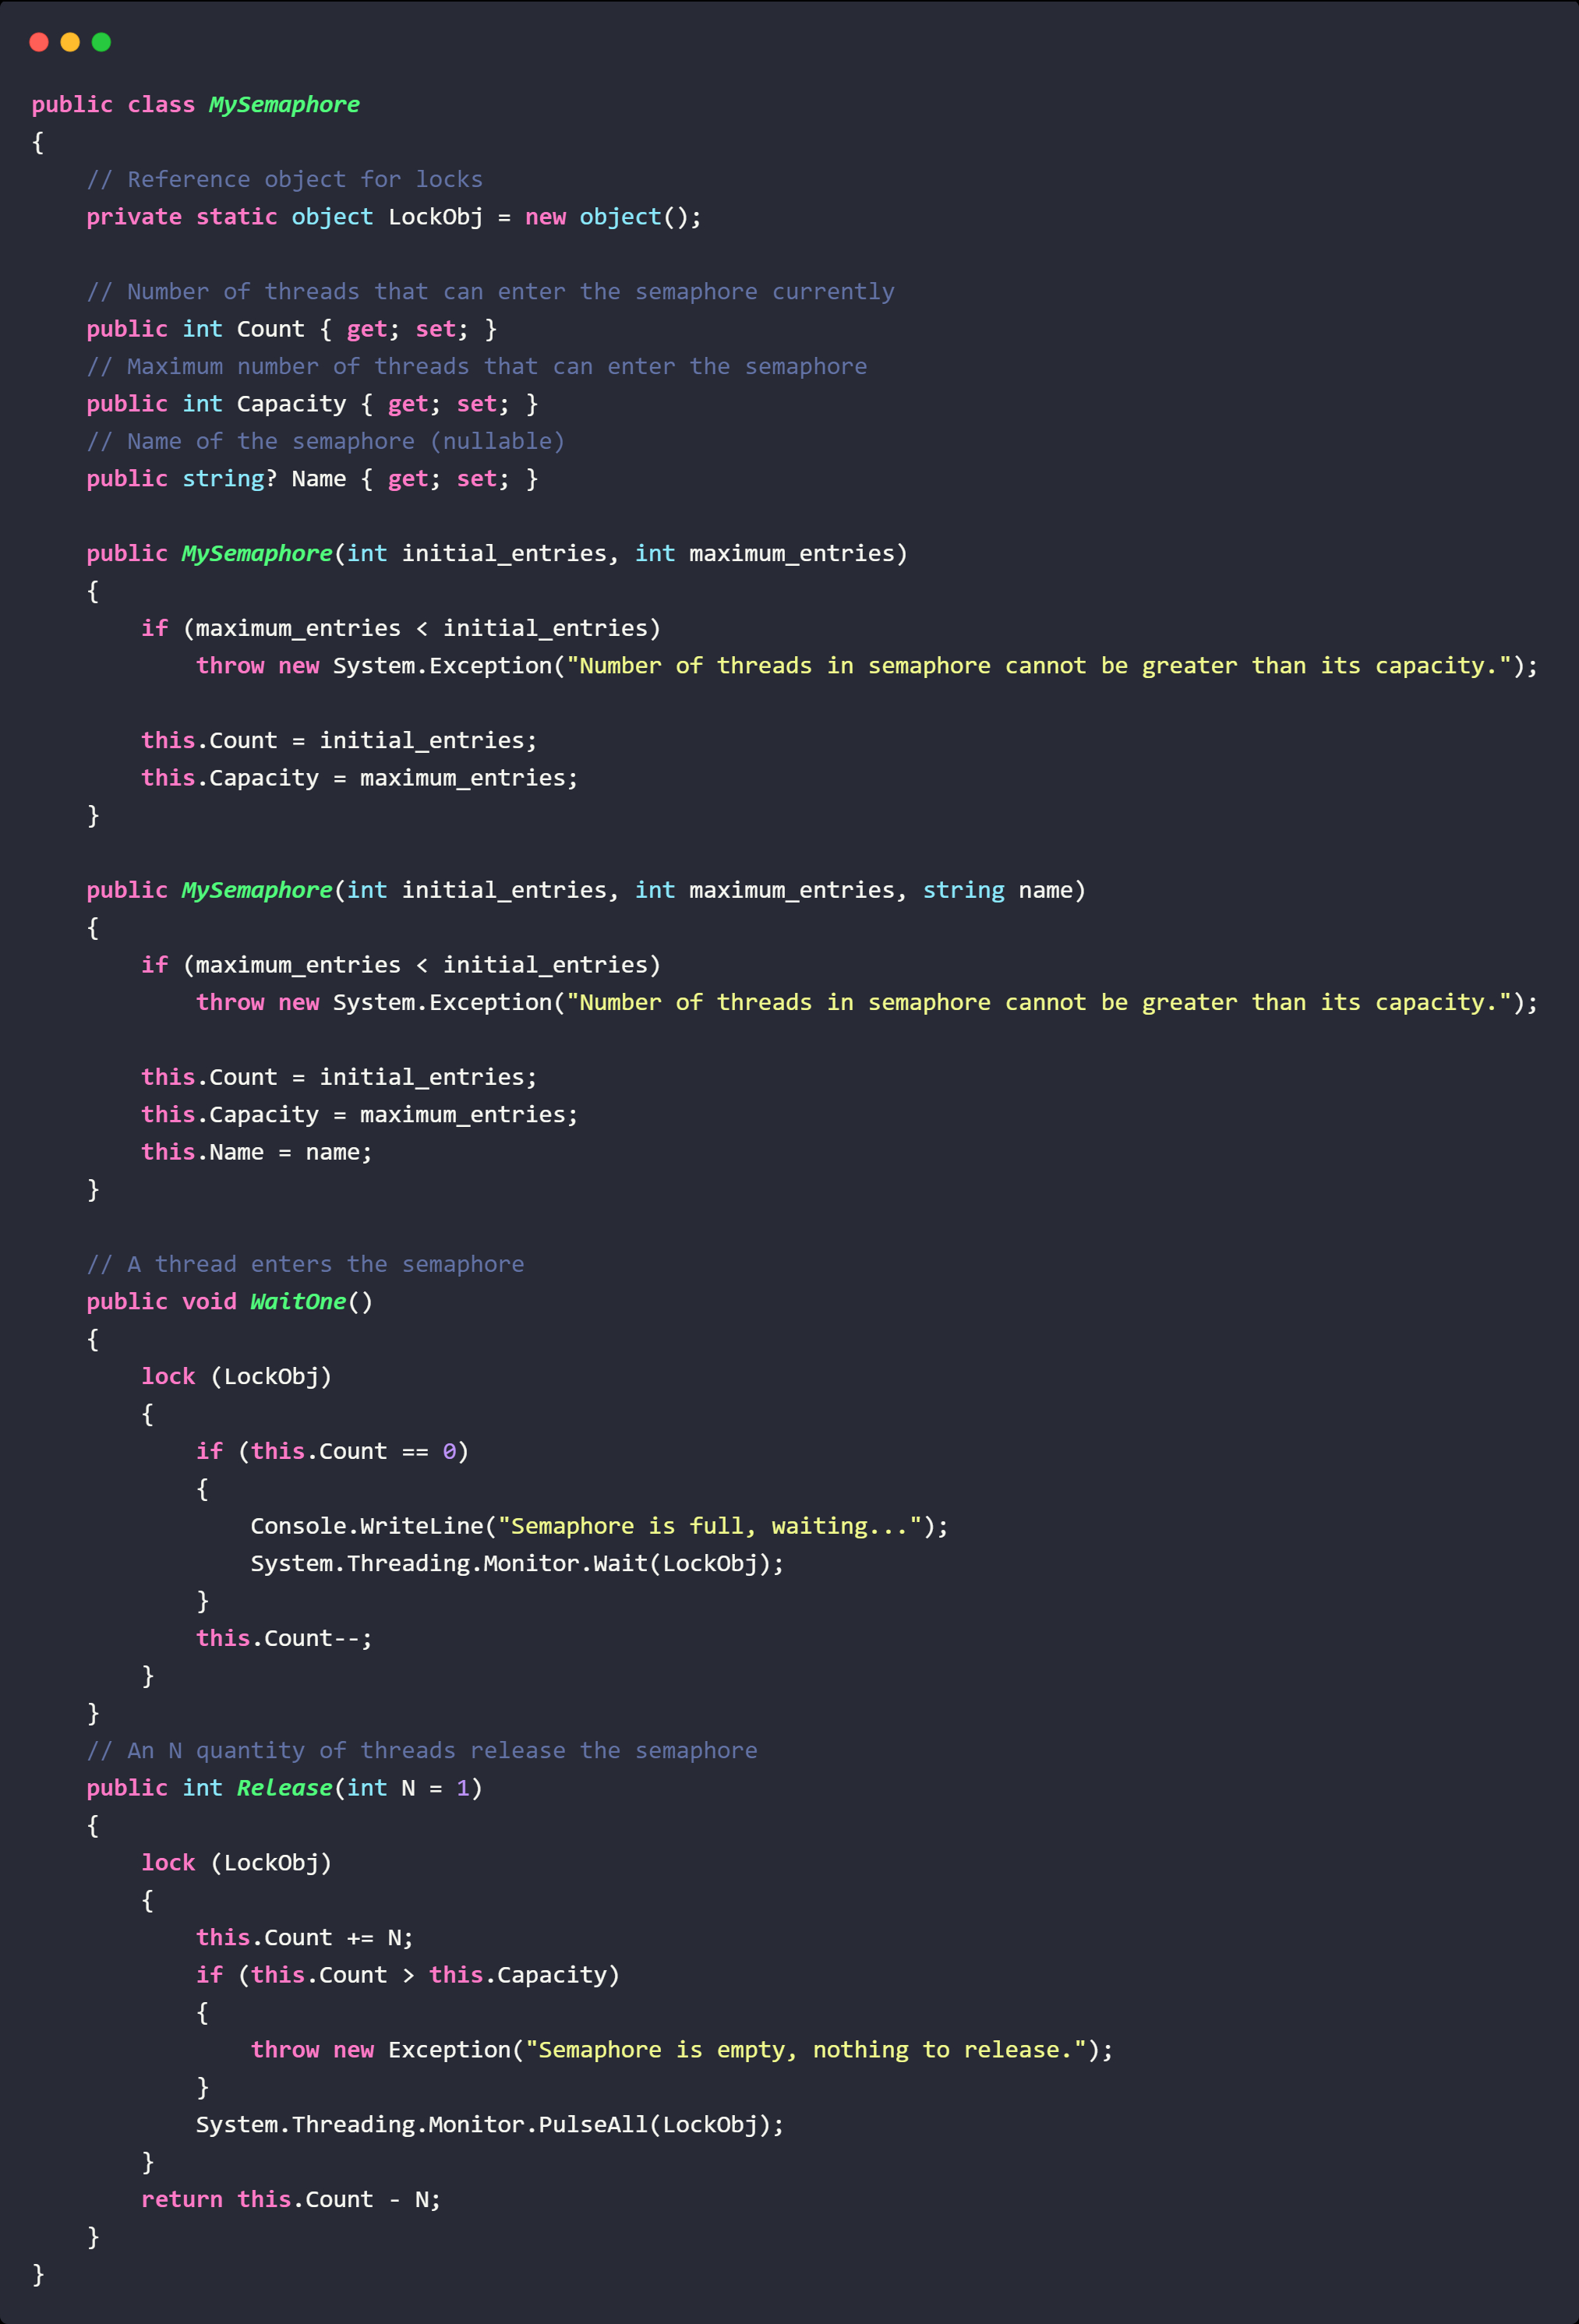
\includegraphics[width=15cm]{MySemaphore.jpg}

\subsection{Barriers en C\#}

Permite que múltiples tareas trabajen de manera cooperativa en un algoritmo en paralelo a través de múltiples fases.

En esta sincronización de barrera, tenemos varios subprocesos que trabajan en un solo algoritmo. El algoritmo funciona en fases. Todos los subprocesos deben completar la fase 1 y luego pueden continuar con la fase 2. Hasta que todos los subprocesos no completen la fase 1, todos los subprocesos deben esperar a que todos los subprocesos lleguen a la fase 1.

\subsection{Countdowns en C\#}

Representa una primitiva de sincronización que emite una señal cuando su cuenta llega a cero.

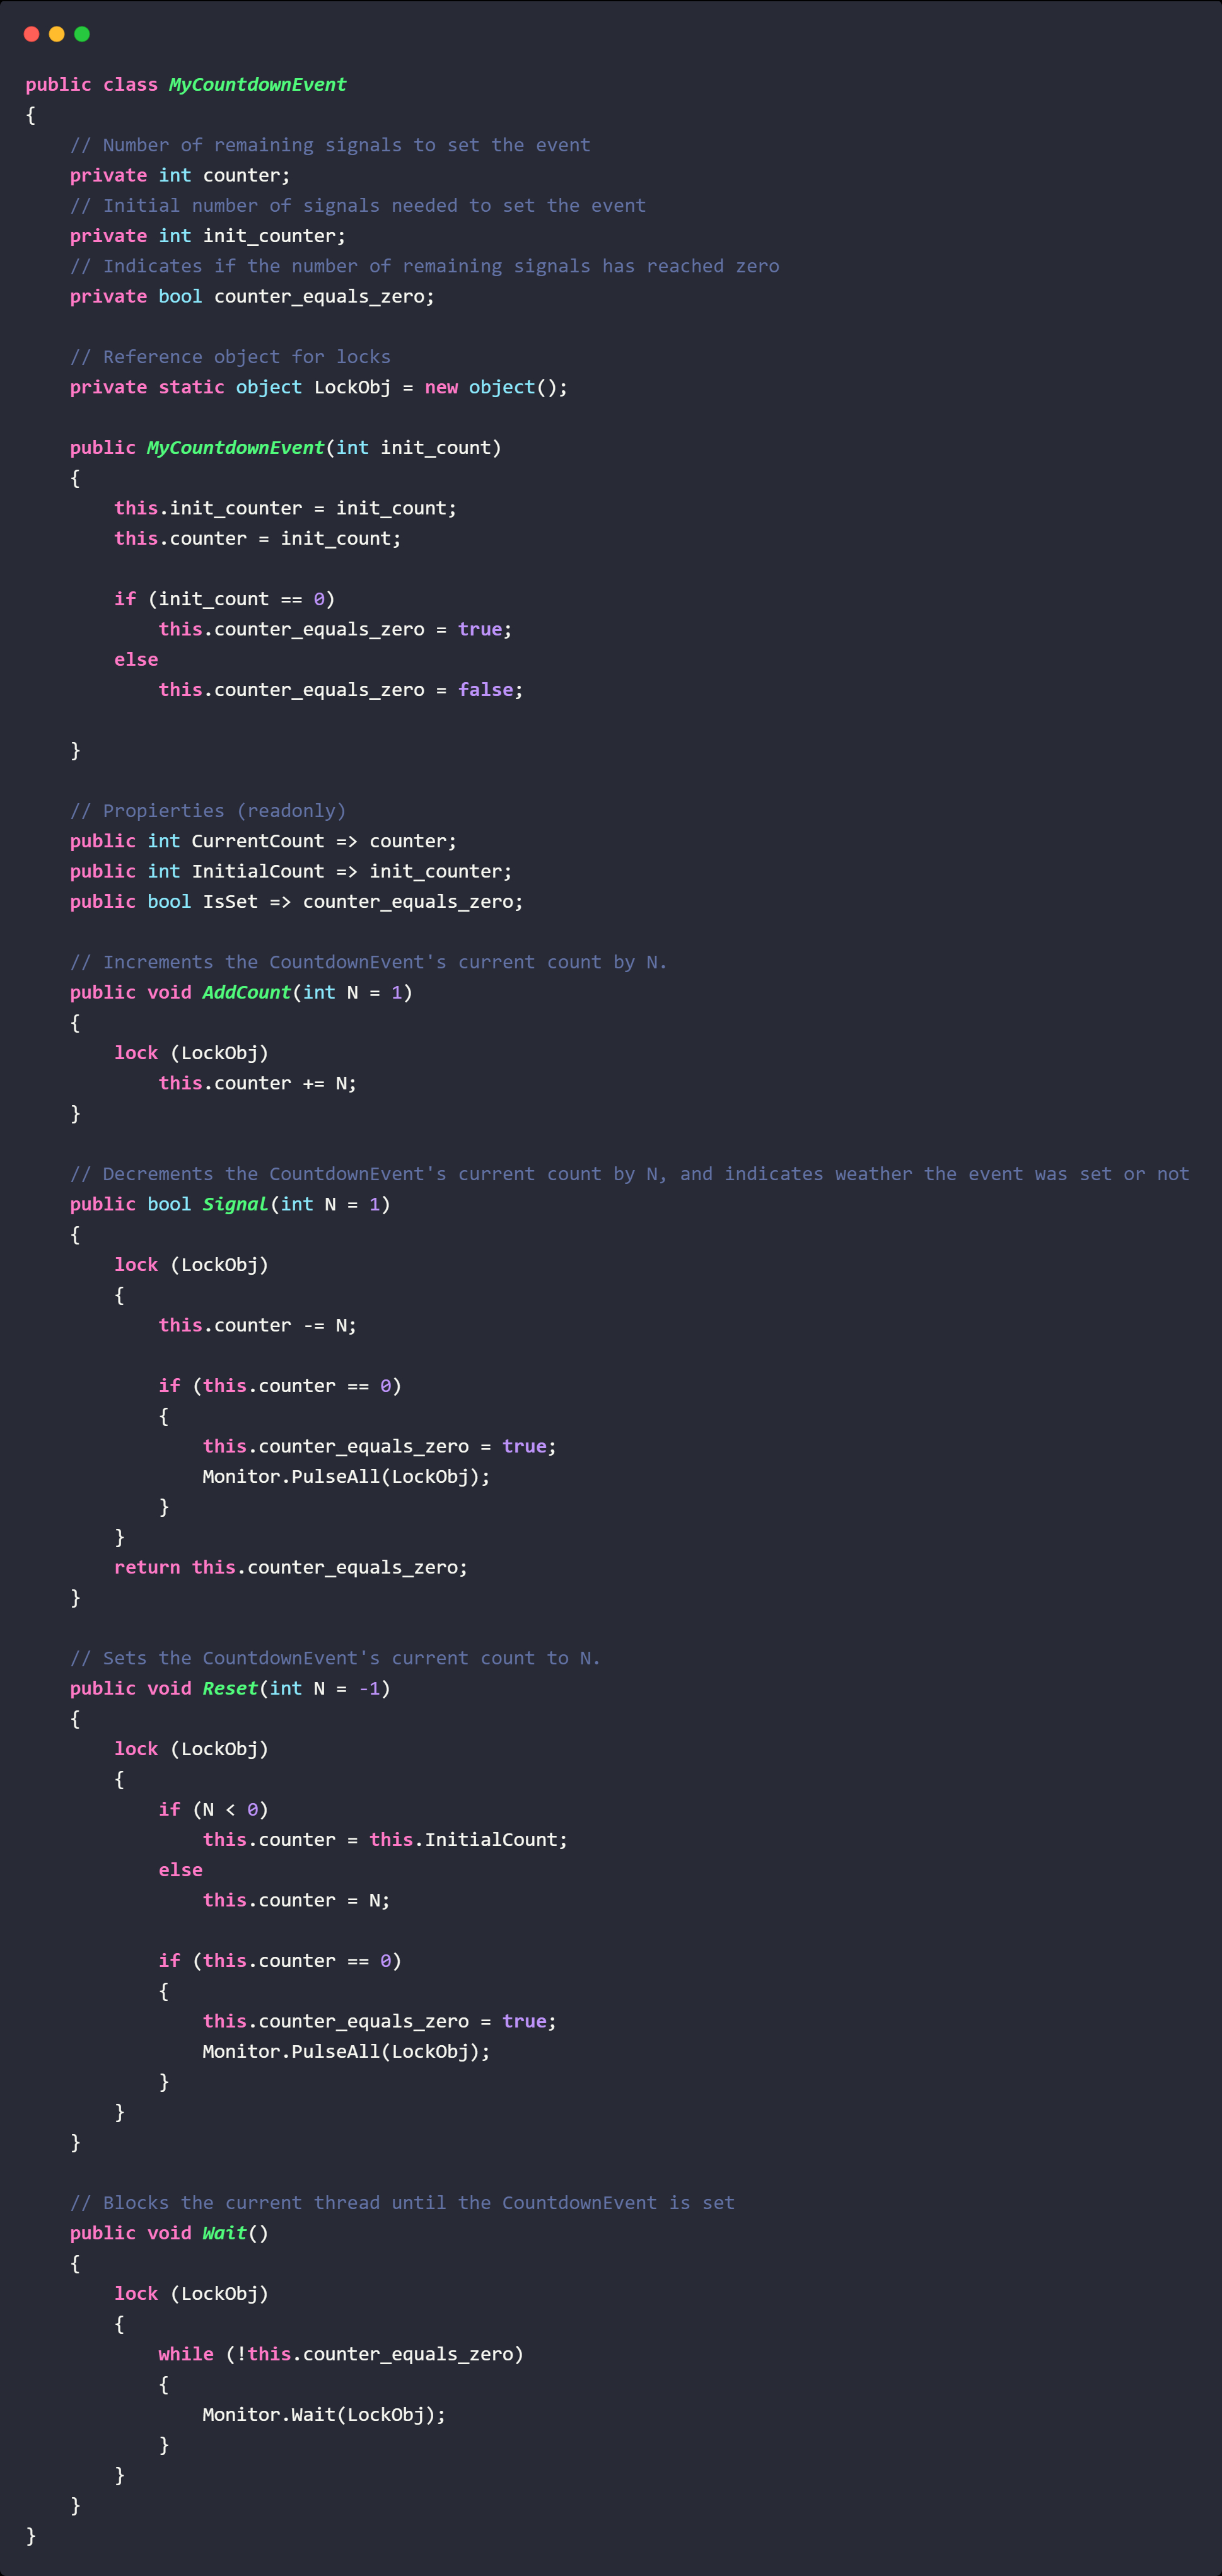
\includegraphics[width=15cm]{MyCountdownEvent.jpg}

\subsection{Propuesta en Go para la sincronización en la concurrencia}

\subsection{Solución a los filósofos}

\subsubsection{Go}

\subsubsection{C\#}

\subsubsection{Comparaci\'on}
%----------------------------------------------------------------------------------------

\begin{thebibliography}
	a
	\bibitem{katrib} Miguel Katrib. \emph{Empezar a programar. Un enfoque multiparadigma con C\#}. 
	Editorial UH.
	2020.
	La Habana.
	\bibitem{microsoft} \href{https://learn.microsoft.com/en-us/dotnet/api/system.threading?view=net-7.0}{Microsoft Learn: System.Threading Namespace in .NET}
\end{thebibliography}

\end{document}
